%
% File acl2020.tex
%
%% Based on the style files for ACL 2020, which were
%% Based on the style files for ACL 2018, NAACL 2018/19, which were
%% Based on the style files for ACL-2015, with some improvements
%%  taken from the NAACL-2016 style
%% Based on the style files for ACL-2014, which were, in turn,
%% based on ACL-2013, ACL-2012, ACL-2011, ACL-2010, ACL-IJCNLP-2009,
%% EACL-2009, IJCNLP-2008...
%% Based on the style files for EACL 2006 by 
%%e.agirre@ehu.es or Sergi.Balari@uab.es
%% and that of ACL 08 by Joakim Nivre and Noah Smith

\documentclass[11pt,a4paper]{article}
\usepackage[hyperref]{acl2020}
\usepackage{times}
\usepackage{latexsym}
\usepackage{graphicx}
\renewcommand{\UrlFont}{\ttfamily\small}
\usepackage[utf8]{inputenc}
\usepackage{amsmath}
\usepackage{amsfonts}
\newcommand{\e}[1]{{\mathbb E}\left[ #1 \right]}

% This is not strictly necessary, and may be commented out,
% but it will improve the layout of the manuscript,
% and will typically save some space.
\usepackage{microtype}

%\aclfinalcopy % Uncomment this line for the final submission
%\def\aclpaperid{***} %  Enter the acl Paper ID here

%\setlength\titlebox{5cm}
% You can expand the titlebox if you need extra space
% to show all the authors. Please do not make the titlebox
% smaller than 5cm (the original size); we will check this
% in the camera-ready version and ask you to change it back.

\newcommand\BibTeX{B\textsc{ib}\TeX}

\title{Charlie: Charts for Language Insight Extraction}

\author{First Author \\
  Affiliation / Address line 1 \\
  Affiliation / Address line 2 \\
  Affiliation / Address line 3 \\
  \texttt{email@domain} \\\And
  Second Author \\
  Affiliation / Address line 1 \\
  Affiliation / Address line 2 \\
  Affiliation / Address line 3 \\
  \texttt{email@domain} \\}

\date{}

\begin{document}
\maketitle
\begin{abstract}
Charlie, Charts for Language Insights Extraction, is an interactive tool in the form of a dashboard. Its main purpose is to enable the understanding and summarization regarding a collection of textual dialogs (chats). By leveraging a unique composition of textual representation, unsupervised clustering, and supervised explainable classification, Charlie provides useful and condensed insights that can result in a variety of applications, particularly for the Customer Experience area. For example, it could considerably reduce time and costs of chatbot creation by detecting customers’ problems faster, without the need of human annotation. The solution was developed using a conversation database provided by one of the ten largest banks in Brazil. The main topics regard bill query, copy of contract, debt transfer, credit card or collection assistance, for example. Charlie is able to display clusters of conversations, provide global information of each cluster in the form of word clouds and t-SNE embedding projection. It also gives a detailed local interactive view of the conversations inside each cluster, showing meaningful dialog parts as well as the original bank classification. In some cases, Charlie outperformed the bank's classification system, putting together in the correct group texts that had been originally misclassified by the bank.

\end{abstract}


\section{Introduction}

The rise of customer service solutions through text dialogs brings along the opportunity of understanding and summarizing issues much easily than through audio data. This is because audio files contain extra information that adds complexity to the process, like pauses, intonation, external noise, accent, pitch, etc. Moreover, they occupy much more memory than text files. Conversely, text data can be interpreted and processed by most of programming languages, which facilitates processes of data analysis. However, like any human form of communication, textual dialogs are quite unstructured, and therefore need to be reorganized to better enable analyses. Thus, we begin by describing the typical dialog structure found in our database.

\begin{figure}
    \centering
    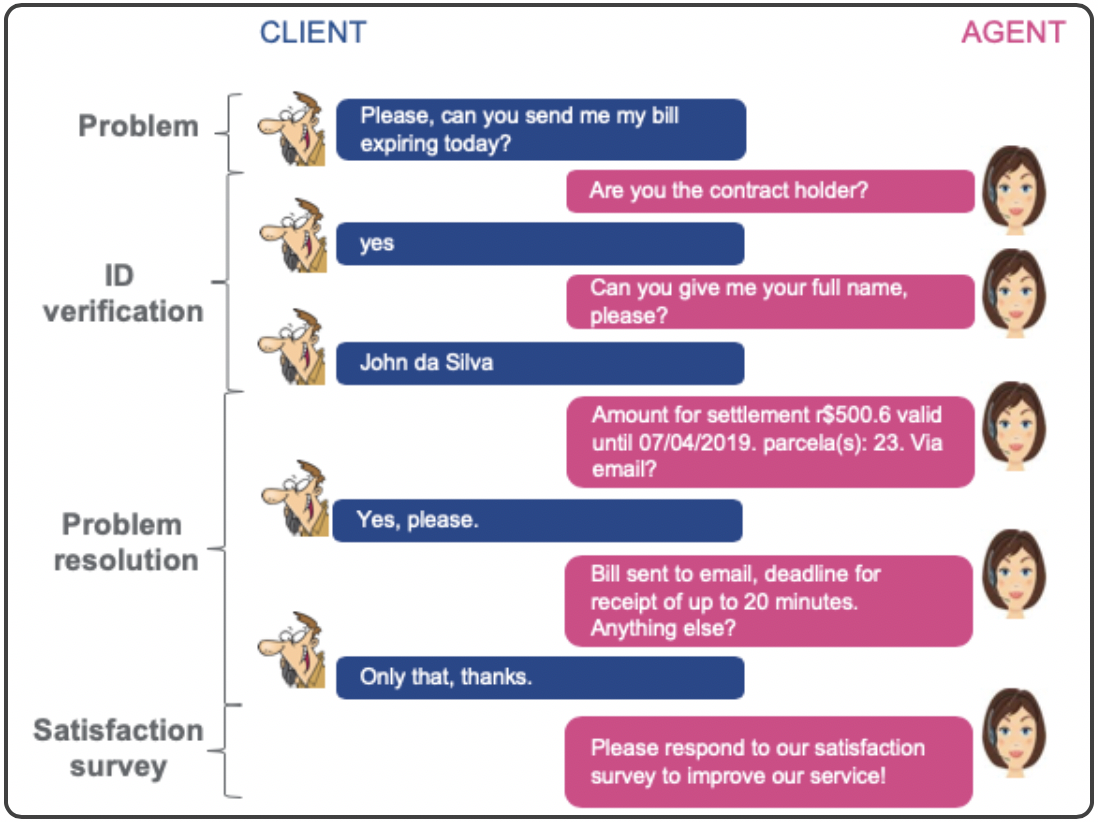
\includegraphics[width=0.5\textwidth]{figures/dialogue_description.png}
    \caption{Example of conversation between a client and an agent, highlighting the conversation flow and structure.}
    \label{fig:dialog_description}
\end{figure}

The database in use was provided by a financial Brazilian company. The main topics at stake regard bill query, copy of contract, debt transfer, credit card and collection assistance. In this context, the clients are contacting the bank’s customer service to solve a request. Hence, each client’s request can be defined as an \textit{intention}. From the reading of various conversations from different categories, we identified two types of intentions: \textit{simple} and \textit{complex}. \textit{Simple intentions} are characterized by conversations with a simple and common structure. An example is displayed in Fig.\ref{fig:dialog_description}. This kind of dialog generally follows a simple and logical organization, starting with the client problem statement, the client’s ID verification, a step of problem resolution, finalizing with a satisfaction survey. This structure provides a potentially automatable context, in which a bot could substitute human interactions. In contrast, complex intentions define more complex conversations that generally require human intervention to be solved. We can cite for example debt negotiation or collection assistance, topics that require multiple and unpredictable interactions. Naturally, the task of classifying a dialog as being \textit{simple} or \textit{complex} is not only subjective, but also laborious: it would require multiple manual reviewing of a collection of dialogs to determine their complexity. Likewise, the task of categorizing different dialogs accordingly to their respective \textit{intentions} is not clear. For instance, such possible categories are unknown. Although there is a prior knowledge about a few major topics, it is not sufficient to account for all the possible types of requests. 
In this paper, we propose a new tool to help in this task of analyzing a collection of dialogs.

\section{Solution Overview}
\label{lab:overview}

Charlie is an interactive NLP dashboard tool built with the objective of displaying useful information obtained from textual dialog data. Figure \ref{fig:dashboard} ehxibits a static view of Charlie. 
\begin{figure}
    \centering
    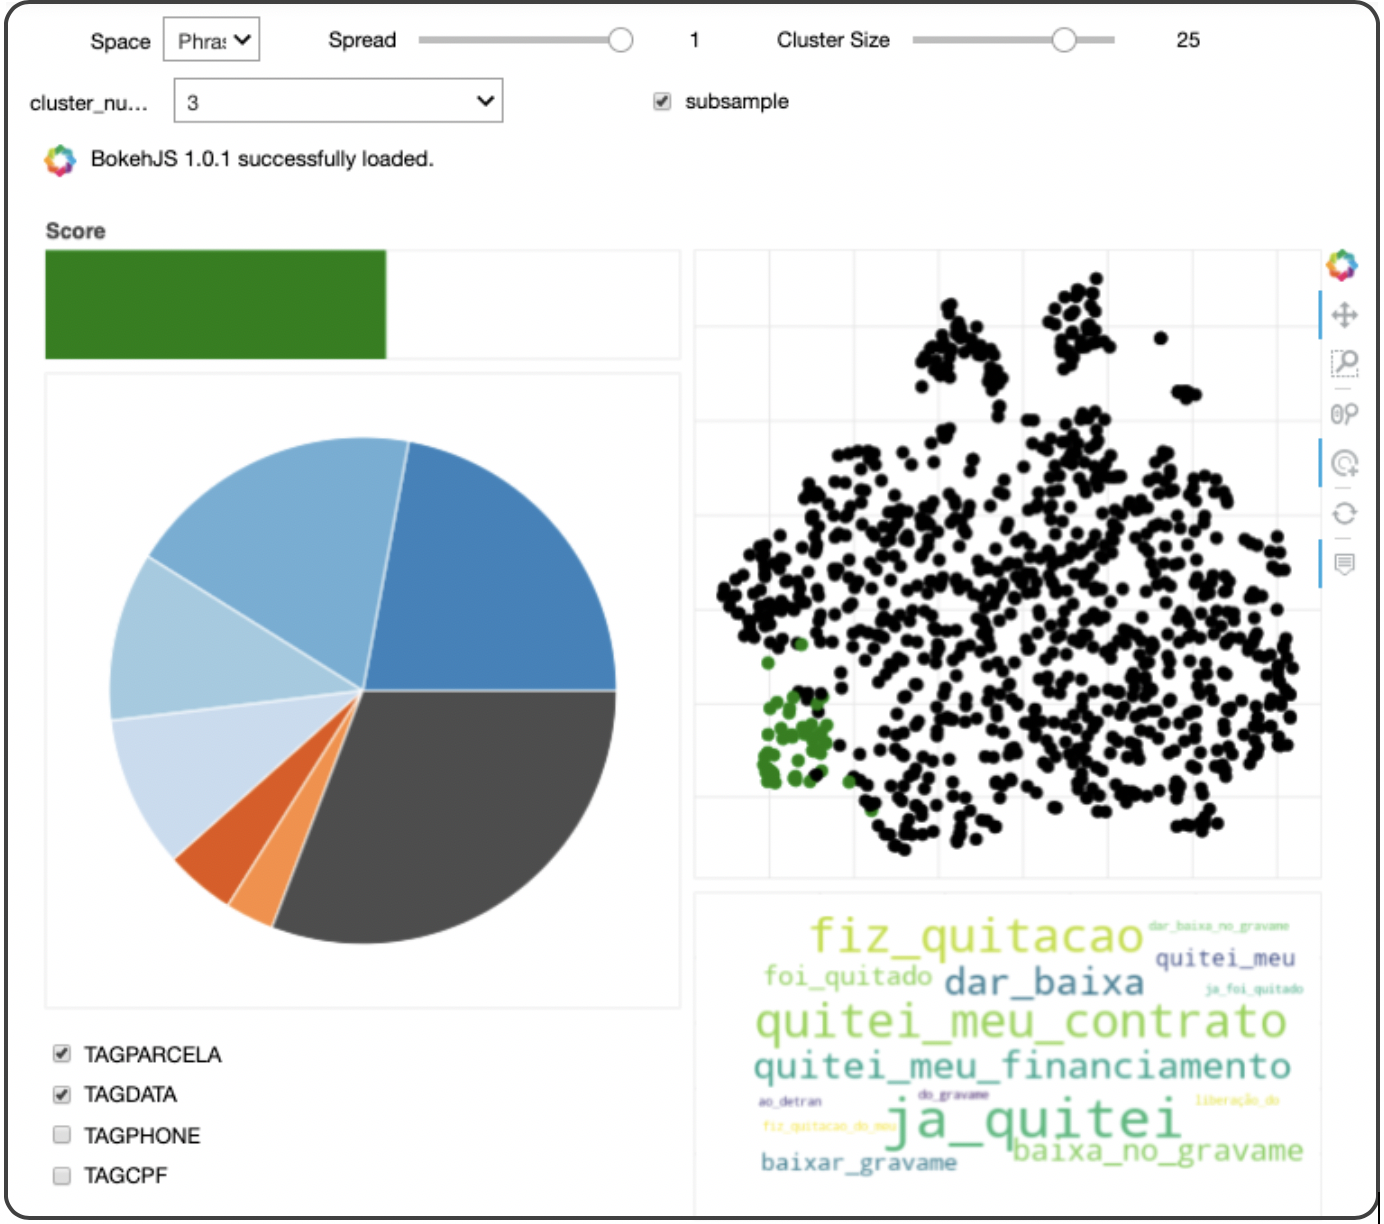
\includegraphics[width=0.5\textwidth]{figures/dashboard.png}
    \caption{Screenshot of Charlie, the dashboard for dialog information extraction}
    \label{fig:dashboard}
\end{figure}
 In this figure there are many different sections, charts and option buttons. 
At the top of Fig. \ref{fig:dashboard} is Charlie’s control panel, where it is possible to select different clusters to scrutinize and choose other customizable options. Below is a list of the items present in Charlie’s control panel:

\begin{itemize}
    \item Score: The silhouette score characterizing the cluster is shown as a green bar at the top left corner of the dashboard. Larger scores mean that the cluster's dialogs are very similar in comparison to out-of-cluster dialogs, and therefore indicates coherent clusters. 
    \item cluster\_num: A list of all clusters is accessible through a drop-down list, ordered by the cluster score. The user can interact with this option to select and analyze different clusters. The ordering is very important, since the highest scoring clusters are promising to show patterns underlying the data, while low-scoring clusters do not provide any insight.
    \item Spread: This parameter takes discrete values from -1 to +1, and is mapped into t-SNE's perplexity parameter. This alias is intended to hide the complexity and build intuition to the user, since the agglomeration of the points changes with this parameter.
    \item Cluster Size: This is an alias to $\frac{1}{N}$ with N the number of clusters. The number of clusters is the real parameter in the clustering algorithm, but it is not really important for the exploratory analysis enabled by Charlie, since only the most relevant clusters should really be assessed. Therefore, we use Cluster Size as the dashboard parameter to ease intuition.
    \item Subsample: The user can choose to observe all the conversations or only a subsample. Depending on the total conversations number and the memory available, we strongly advise the use of this option that selects randomly a subsample of each cluster.
    \item Space: The embedding space. The dashboard directly enables the comparison of distinct textual representations, each with its own corresponding clustering calculated.
    
    On the right of Fig. \ref{fig:dashboard}, is a t-SNE visualization of dialog clusters. In this section, once a cluster is selected, it is possible to observe a highlighted group of dots (each representing a dialog) that have been grouped together according to their semantic content. It is also possible to slide the mouse over any dot and see a preview of the conversation (shown in Figure 4). By sliding it over multiple dots, it is possible to observe similarities in the contexts of the interactions.
\end{itemize}
	
\section{Discovering Dialog Intentions}

We approach the task of identifying \textit{dialog intentions} through the perspective of an unsupervised machine learning problem. We developed a clustering algorithm to find coherent groups of dialogs according to their semantic content.

\subsection{Dialog clustering challenges}
In our setting, clusters are groups of conversations that may fit together because of common characteristics, but the final decision is left to a human user.

Unsupervised learning is generally hard to evaluate \cite{}, with its use cases being very distinct from those of supervised learning \cite{}. Clustering techniques make use of similarity (or distance) metrics to try to group together things that are similar, and separate things that are not similar.



\subsection{Conversation Embeddings}

To enable the dialog clustering, it is necessary to build vector representations that preserve the most relevant and distinguishable aspects of dialogs. To solve this problem, we first applied a preprocessing algorithm to eliminate  interactions with less informative content. For instance, following the typical dialog structure shown in Fig. \ref{fig:dialog_description}, the preprocessing algorithm aims to detect and eliminate interactions that are not part of the "Problem" and "Problem Resolution" stages. The "Problem" stage is the phase in the dialog in which the user states their request. Analogously, the "Problem Resolution" stage is the phase in which the agent provides a solution to the client's request. 

To build the dialog vector representations, we start by building TF-IDF representations for the "Problem Statement" phase. Next, we input these TF-IDF representations into a Neural Network architecture (Fig. \ref{fig:embedding}) to predict a BOW (ref) representation of its respective "Solution". In essence, this model is being trained to build more similar representations for dialogs in which the agent response are similar. The rationale behind this assumption comes from the idea that similar solutions may be a indicative of similar requests. The result of this transformation is an embedded representation of each dialog. 

\begin{figure}
    \centering
    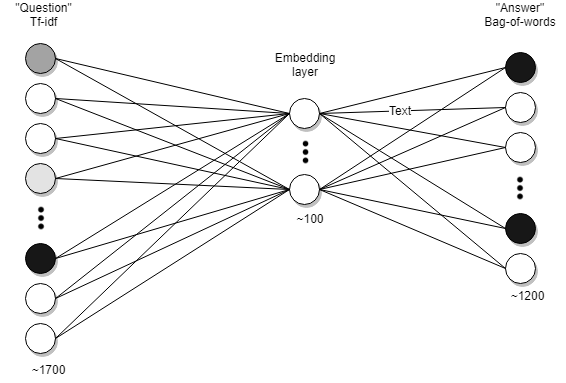
\includegraphics[width=0.5\textwidth]{figures/Embedding.png}
    \caption{Neural network architecture used to build the dialogue embeddings.}
    \label{fig:embedding}
\end{figure}

The hyperparameters we used for training are displayd in Table \ref{tab:hyper}. (talvez falar sobre os hiperparametros, comentar sobre pq usamos apenas 5 epocas e como encontramos min df e max df)

\begin{table}[]
\begin{tabular}{lll}
Optimizer & Adam   \\
Embedding size  &   100     \\
Batch size      &   64   \\
Epochs & 5\\
Minimum Document Frequency & 30\\
Maximum Document Frequency & 99
\end{tabular}
\caption{Hyperparameters}
\label{tab:hyper}
\end{table}

Once the representations have been found, we applied a Gaussian Mixture Model (ref), fitting diagonal covariance matrices to the distribution of points in the space. It is a soft clustering method, and thus assigns probabilities for each point belonging to each cluster. We then applied the t-SNE (ref) algorithm to better visualize the data. 

\section{Validating Clusters and Identifying Relevant Content}

Once the dialogs have been clustered, it is important to understand and explore the resulting groups. We start this analysis by providing an ordering based on the most "coherent" clusters. This can be done through the use of an adaptation of the Silhouette Score (ref), as commented in Section \ref{lab:overview}. Our scoring algorithm can be described as follows:

\begin{enumerate}
    \item Let $a_{i}$ be the average distance of sample \textbf{i} to other samples inside the cluster
    \item Let $b_{i}$ be the average distance of a sample to every sample outside the cluster
    \item $\e{\frac{a_{i}-b_{i}}{max(a_{i},b_{i})}}$ is the proposed score
\end{enumerate}

This algorithm differs from the usual Silhouette Score in two points: First, the usual calculates \textit{b} using only the closest cluster, and second, it also gives a single score for the whole model - applying this different algorithm enables the interpretation of a single cluster.

In addition to this scoring, we can further analyze a cluster's quality by looking at a wordcloud located at the bottom of the panel. A zoomed view of this feature is displayed in Fig. \ref{fig:wordcloud}. Indeed, this visualization enables users to grasp a cluster's general overview, and therefore identify an overall subject for this cluster. Tho build this wordcloud, we used SHAPLEY Values (ref) to identify which terms were more relevant for the model. The resulting word clouds are composed by the most relevant n-grams in the group (separated by an underscore symbol). 

\begin{figure}
    \centering
    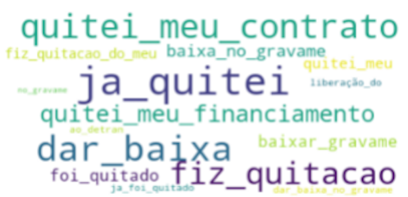
\includegraphics{figures/wordcloud.png}
    \caption{Charlie's wordcloud section.}
    \label{fig:wordcloud}
\end{figure}

\section{Results}

Since the objective of this tool is not to achieve some specific goal or metric, but to assist in the investigation of textual data, we will base our evaluation in comparison to the bank's original classification system. 

\begin{figure}[ht!]
    \centering
    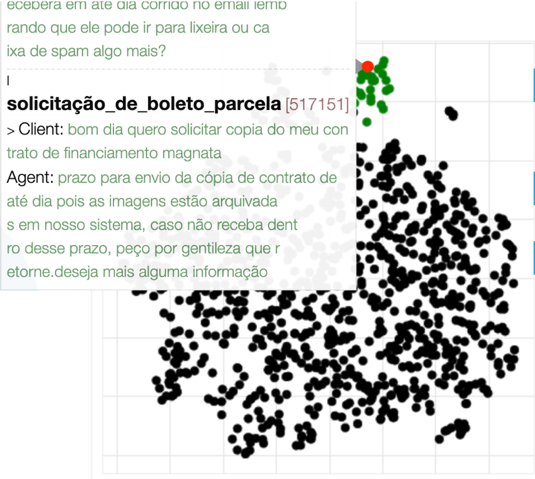
\includegraphics[width=0.4\textwidth]{figures/clustering_section.png}
    \caption{Cluster section: A comparison between the original classification and the actual dialog content.}
    \label{fig:cluster}
\end{figure}

Fig. \ref{fig:cluster} exhibits the set of conversations represented by dots. The green dots indicate the cluster that is being analyzed at the moment. The red dot is the dialog that is being displayed alongside. The title of the dialog is the previous adopted classification. The text in green is a preview of the part of the dialog in which the user express their \textit{intention}.  

\section{Identifying Typical Conversation Parts}

(grafico de pizza)
\begin{itemize}
    \item Desceibe the problem of identifying important parts of the dialog
    \item used technique to solve this problem
    \item some applications of this feature
\end{itemize}


\section{Conclusions}

\section{Future Work}




% \subsection{File Format}
% \label{sect:pdf}

% For the production of the electronic manuscript you must use Adobe's Portable Document Format (PDF).
% Please make sure that your PDF file includes all the necessary fonts (especially tree diagrams, symbols, and fonts with Asian characters).
% When you print or create the PDF file, there is usually an option in your printer setup to include none, all or just non-standard fonts.
% Please make sure that you select the option of including ALL the fonts.
% \textbf{Before sending it, test your PDF by printing it from a computer different from the one where it was created.}
% Moreover, some word processors may generate very large PDF files, where each page is rendered as an image.
% Such images may reproduce poorly.
% In this case, try alternative ways to obtain the PDF.
% One way on some systems is to install a driver for a postscript printer, send your document to the printer specifying ``Output to a file'', then convert the file to PDF.

% It is of utmost importance to specify the \textbf{A4 format} (21 cm x 29.7 cm) when formatting the paper.
% Print-outs of the PDF file on A4 paper should be identical to the hardcopy version.
% If you cannot meet the above requirements about the production of your electronic submission, please contact the publication chairs as soon as possible.

% \paragraph{\LaTeX-specific details:}
% PDF files are usually produced from \LaTeX{} using the \texttt{\small pdflatex} command.
% If your version of \LaTeX{} produces Postscript files, \texttt{\small ps2pdf} or \texttt{\small dvipdf} can convert these to PDF.
% To ensure A4 format in \LaTeX, use the command {\small\verb|\special{papersize=210mm,297mm}|}
% in the \LaTeX{} preamble (below the {\small\verb|\usepackage|} commands) and use \texttt{\small dvipdf} and/or \texttt{\small pdflatex}; or specify \texttt{\small -t a4} when working with \texttt{\small dvips}.

% \subsection{Layout}
% \label{ssec:layout}

% Format manuscripts two columns to a page, in the manner these
% instructions are formatted.
% The exact dimensions for a page on A4 paper are:

% \begin{itemize}
% \item Left and right margins: 2.5 cm
% \item Top margin: 2.5 cm
% \item Bottom margin: 2.5 cm
% \item Column width: 7.7 cm
% \item Column height: 24.7 cm
% \item Gap between columns: 0.6 cm
% \end{itemize}

% \noindent Papers should not be submitted on any other paper size.
% If you cannot meet the above requirements about the production of your electronic submission, please contact the publication chairs above as soon as possible.

% \subsection{Fonts}

% For reasons of uniformity, Adobe's \textbf{Times Roman} font should be used.
% If Times Roman is unavailable, you may use Times New Roman or \textbf{Computer Modern Roman}.

% Table~\ref{font-table} specifies what font sizes and styles must be used for each type of text in the manuscript.

% \begin{table}
% \centering
% \begin{tabular}{lrl}
% \hline \textbf{Type of Text} & \textbf{Font Size} & \textbf{Style} \\ \hline
% paper title & 15 pt & bold \\
% author names & 12 pt & bold \\
% author affiliation & 12 pt & \\
% the word ``Abstract'' & 12 pt & bold \\
% section titles & 12 pt & bold \\
% subsection titles & 11 pt & bold \\
% document text & 11 pt  &\\
% captions & 10 pt & \\
% abstract text & 10 pt & \\
% bibliography & 10 pt & \\
% footnotes & 9 pt & \\
% \hline
% \end{tabular}
% \caption{\label{font-table} Font guide. }
% \end{table}

% \paragraph{\LaTeX-specific details:}
% To use Times Roman in \LaTeX2e{}, put the following in the preamble:
% \begin{quote}
% \small
% \begin{verbatim}
% \usepackage{times}
% \usepackage{latexsym}
% \end{verbatim}
% \end{quote}


% \subsection{Ruler}
% A printed ruler (line numbers in the left and right margins of the article) should be presented in the version submitted for review, so that reviewers may comment on particular lines in the paper without circumlocution.
% The presence or absence of the ruler should not change the appearance of any other content on the page.
% The camera ready copy should not contain a ruler.

% \paragraph{Reviewers:}
% note that the ruler measurements may not align well with lines in the paper -- this turns out to be very difficult to do well when the paper contains many figures and equations, and, when done, looks ugly.
% In most cases one would expect that the approximate location will be adequate, although you can also use fractional references (\emph{e.g.}, this line ends at mark $295.5$).

% \paragraph{\LaTeX-specific details:}
% The style files will generate the ruler when {\small\verb|\aclfinalcopy|} is commented out, and remove it otherwise.

% \subsection{Title and Authors}
% \label{ssec:title-authors}

% Center the title, author's name(s) and affiliation(s) across both columns.
% Do not use footnotes for affiliations.
% Place the title centered at the top of the first page, in a 15-point bold font.
% Long titles should be typed on two lines without a blank line intervening.
% Put the title 2.5 cm from the top of the page, followed by a blank line, then the author's names(s), and the affiliation on the following line.
% Do not use only initials for given names (middle initials are allowed).
% Do not format surnames in all capitals (\emph{e.g.}, use ``Mitchell'' not ``MITCHELL'').
% Do not format title and section headings in all capitals except for proper names (such as ``BLEU'') that are
% conventionally in all capitals.
% The affiliation should contain the author's complete address, and if possible, an electronic mail address.

% The title, author names and addresses should be completely identical to those entered to the electronical paper submission website in order to maintain the consistency of author information among all publications of the conference.
% If they are different, the publication chairs may resolve the difference without consulting with you; so it is in your own interest to double-check that the information is consistent.

% Start the body of the first page 7.5 cm from the top of the page.
% \textbf{Even in the anonymous version of the paper, you should maintain space for names and addresses so that they will fit in the final (accepted) version.}


% \subsection{Abstract}
% Use two-column format when you begin the abstract.
% Type the abstract at the beginning of the first column.
% The width of the abstract text should be smaller than the
% width of the columns for the text in the body of the paper by 0.6 cm on each side.
% Center the word \textbf{Abstract} in a 12 point bold font above the body of the abstract.
% The abstract should be a concise summary of the general thesis and conclusions of the paper.
% It should be no longer than 200 words.
% The abstract text should be in 10 point font.

% \subsection{Text}
% Begin typing the main body of the text immediately after the abstract, observing the two-column format as shown in the present document.

% Indent 0.4 cm when starting a new paragraph.

% \subsection{Sections}

% Format section and subsection headings in the style shown on the present document.
% Use numbered sections (Arabic numerals) to facilitate cross references.
% Number subsections with the section number and the subsection number separated by a dot, in Arabic numerals.

% \subsection{Footnotes}
% Put footnotes at the bottom of the page and use 9 point font.
% They may be numbered or referred to by asterisks or other symbols.\footnote{This is how a footnote should appear.}
% Footnotes should be separated from the text by a line.\footnote{Note the line separating the footnotes from the text.}

% \subsection{Graphics}

% Place figures, tables, and photographs in the paper near where they are first discussed, rather than at the end, if possible.
% Wide illustrations may run across both columns.
% Color is allowed, but adhere to Section~\ref{ssec:accessibility}'s guidelines on accessibility.

% \paragraph{Captions:}
% Provide a caption for every illustration; number each one sequentially in the form:
% ``Figure 1. Caption of the Figure.''
% ``Table 1. Caption of the Table.''
% Type the captions of the figures and tables below the body, using 10 point text.
% Captions should be placed below illustrations.
% Captions that are one line are centered (see Table~\ref{font-table}).
% Captions longer than one line are left-aligned (see Table~\ref{tab:accents}).

% \begin{table}
% \centering
% \begin{tabular}{lc}
% \hline
% \textbf{Command} & \textbf{Output}\\
% \hline
% \verb|{\"a}| & {\"a} \\
% \verb|{\^e}| & {\^e} \\
% \verb|{\`i}| & {\`i} \\ 
% \verb|{\.I}| & {\.I} \\ 
% \verb|{\o}| & {\o} \\
% \verb|{\'u}| & {\'u}  \\ 
% \verb|{\aa}| & {\aa}  \\\hline
% \end{tabular}
% \begin{tabular}{lc}
% \hline
% \textbf{Command} & \textbf{Output}\\
% \hline
% \verb|{\c c}| & {\c c} \\ 
% \verb|{\u g}| & {\u g} \\ 
% \verb|{\l}| & {\l} \\ 
% \verb|{\~n}| & {\~n} \\ 
% \verb|{\H o}| & {\H o} \\ 
% \verb|{\v r}| & {\v r} \\ 
% \verb|{\ss}| & {\ss} \\
% \hline
% \end{tabular}
% \caption{Example commands for accented characters, to be used in, \emph{e.g.}, \BibTeX\ names.}\label{tab:accents}
% \end{table}

% \paragraph{\LaTeX-specific details:}
% The style files are compatible with the caption and subcaption packages; do not add optional arguments.
% \textbf{Do not override the default caption sizes.}


% \subsection{Hyperlinks}
% Within-document and external hyperlinks are indicated with Dark Blue text, Color Hex \#000099.

% \subsection{Citations}
% Citations within the text appear in parentheses as~\citep{Gusfield:97} or, if the author's name appears in the text itself, as \citet{Gusfield:97}.
% Append lowercase letters to the year in cases of ambiguities.  
% Treat double authors as in~\citep{Aho:72}, but write as in~\citep{Chandra:81} when more than two authors are involved. Collapse multiple citations as in~\citep{Gusfield:97,Aho:72}. 

% Refrain from using full citations as sentence constituents.
% Instead of
% \begin{quote}
%   ``\citep{Gusfield:97} showed that ...''
% \end{quote}
% write
% \begin{quote}
% ``\citet{Gusfield:97} showed that ...''
% \end{quote}

% \begin{table*}
% \centering
% \begin{tabular}{lll}
% \hline
% \textbf{Output} & \textbf{natbib command} & \textbf{Old ACL-style command}\\
% \hline
% \citep{Gusfield:97} & \small\verb|\citep| & \small\verb|\cite| \\
% \citealp{Gusfield:97} & \small\verb|\citealp| & no equivalent \\
% \citet{Gusfield:97} & \small\verb|\citet| & \small\verb|\newcite| \\
% \citeyearpar{Gusfield:97} & \small\verb|\citeyearpar| & \small\verb|\shortcite| \\
% \hline
% \end{tabular}
% \caption{\label{citation-guide}
% Citation commands supported by the style file.
% The style is based on the natbib package and supports all natbib citation commands.
% It also supports commands defined in previous ACL style files for compatibility.
% }
% \end{table*}

% \paragraph{\LaTeX-specific details:}
% Table~\ref{citation-guide} shows the syntax supported by the style files.
% We encourage you to use the natbib styles.
% You can use the command {\small\verb|\citet|} (cite in text) to get ``author (year)'' citations as in \citet{Gusfield:97}.
% You can use the command {\small\verb|\citep|} (cite in parentheses) to get ``(author, year)'' citations as in \citep{Gusfield:97}.
% You can use the command {\small\verb|\citealp|} (alternative cite without  parentheses) to get ``author year'' citations (which is useful for  using citations within parentheses, as in \citealp{Gusfield:97}).


% \subsection{References}
% Gather the full set of references together under the heading \textbf{References}; place the section before any Appendices. 
% Arrange the references alphabetically by first author, rather than by order of occurrence in the text.

% Provide as complete a citation as possible, using a consistent format, such as the one for \emph{Computational Linguistics\/} or the one in the  \emph{Publication Manual of the American 
% Psychological Association\/}~\citep{APA:83}.
% Use full names for authors, not just initials.

% Submissions should accurately reference prior and related work, including code and data.
% If a piece of prior work appeared in multiple venues, the version that appeared in a refereed, archival venue should be referenced.
% If multiple versions of a piece of prior work exist, the one used by the authors should be referenced.
% Authors should not rely on automated citation indices to provide accurate references for prior and related work.

% The following text cites various types of articles so that the references section of the present document will include them.
% \begin{itemize}
% \item Example article in journal: \citep{Ando2005}.
% \item Example article in proceedings, with location: \citep{borschinger-johnson-2011-particle}.
% \item Example article in proceedings, without location: \citep{andrew2007scalable}.
% \item Example arxiv paper: \citep{rasooli-tetrault-2015}. 
% \end{itemize}


% \paragraph{\LaTeX-specific details:}
% The \LaTeX{} and Bib\TeX{} style files provided roughly follow the American Psychological Association format.
% If your own bib file is named \texttt{\small acl2020.bib}, then placing the following before any appendices in your \LaTeX{}  file will generate the references section for you:
% \begin{quote}\small
% \verb|\bibliographystyle{acl_natbib}|\\
% \verb|\bibliography{acl2020}|
% \end{quote}

% You can obtain the complete ACL Anthology as a Bib\TeX\ file from \url{https://aclweb.org/anthology/anthology.bib.gz}.
% To include both the anthology and your own bib file, use the following instead of the above.
% \begin{quote}\small
% \verb|\bibliographystyle{acl_natbib}|\\
% \verb|\bibliography{anthology,acl2020}|
% \end{quote}


% \subsection{Digital Object Identifiers}
% As part of our work to make ACL materials more widely used and cited outside of our discipline, ACL has registered as a CrossRef member, as a registrant of Digital Object Identifiers (DOIs), the standard for registering permanent URNs for referencing scholarly materials.

% All camera-ready references are required to contain the appropriate DOIs (or as a second resort, the hyperlinked ACL Anthology Identifier) to all cited works.
% Appropriate records should be found for most materials in the current ACL Anthology at \url{http://aclanthology.info/}.
% As examples, we cite \citep{goodman-etal-2016-noise} to show you how papers with a DOI will appear in the bibliography.
% We cite \citep{harper-2014-learning} to show how papers without a DOI but with an ACL Anthology Identifier will appear in the bibliography.

% \paragraph{\LaTeX-specific details:}
% Please ensure that you use Bib\TeX\ records that contain DOI or URLs for any of the ACL materials that you reference.
% If the Bib\TeX{} file contains DOI fields, the paper title in the references section will appear as a hyperlink to the DOI, using the hyperref \LaTeX{} package.


% \subsection{Appendices}
% Appendices, if any, directly follow the text and the
% references (but only in the camera-ready; see Appendix~\ref{sec:appendix}).
% Letter them in sequence and provide an informative title:
% \textbf{Appendix A. Title of Appendix}.

% \section{Accessibility}
% \label{ssec:accessibility}

% In an effort to accommodate people who are color-blind (as well as those printing to paper), grayscale readability is strongly encouraged.
% Color is not forbidden, but authors should ensure that tables and figures do not rely solely on color to convey critical distinctions.
% A simple criterion:
% All curves and points in your figures should be clearly distinguishable without color.

% \section{Translation of non-English Terms}

% It is also advised to supplement non-English characters and terms with appropriate transliterations and/or translations since not all readers understand all such characters and terms.
% Inline transliteration or translation can be represented in the order of:
% \begin{center}
% \begin{tabular}{c}
% original-form \\
% transliteration \\
% ``translation''
% \end{tabular}
% \end{center}

% \section{\LaTeX{} Compilation Issues}
% You may encounter the following error during compilation: 
% \begin{quote}
% {\small\verb|\pdfendlink|} ended up in different nesting level than {\small\verb|\pdfstartlink|}.
% \end{quote}
% This happens when \texttt{\small pdflatex} is used and a citation splits across a page boundary.
% To fix this, the style file contains a patch consisting of two lines:
% (1) {\small\verb|\RequirePackage{etoolbox}|} (line 455 in \texttt{\small acl2020.sty}), and
% (2) A long line below (line 456 in \texttt{\small acl2020.sty}).

% If you still encounter compilation issues even with the patch enabled, disable the patch by commenting the two lines, and then disable the \texttt{\small hyperref} package by loading the style file with the \texttt{\small nohyperref} option:

% \noindent
% {\small\verb|\usepackage[nohyperref]{acl2020}|}

% \noindent
% Then recompile, find the problematic citation, and rewrite the sentence containing the citation. (See, {\em e.g.}, \url{http://tug.org/errors.html})

% \section*{Acknowledgments}

% The acknowledgments should go immediately before the references. Do not number the acknowledgments section.
% Do not include this section when submitting your paper for review.

% \bibliography{anthology,acl2020}
% \bibliographystyle{acl_natbib}

% \appendix

% \section{Appendices}
% \label{sec:appendix}
% Appendices are material that can be read, and include lemmas, formulas, proofs, and tables that are not critical to the reading and understanding of the paper. 
% Appendices should be \textbf{uploaded as supplementary material} when submitting the paper for review.
% Upon acceptance, the appendices come after the references, as shown here.

% \paragraph{\LaTeX-specific details:}
% Use {\small\verb|\appendix|} before any appendix section to switch the section numbering over to letters.


% \section{Supplemental Material}
% \label{sec:supplemental}
% Submissions may include non-readable supplementary material used in the work and described in the paper.
% Any accompanying software and/or data should include licenses and documentation of research review as appropriate.
% Supplementary material may report preprocessing decisions, model parameters, and other details necessary for the replication of the experiments reported in the paper.
% Seemingly small preprocessing decisions can sometimes make a large difference in performance, so it is crucial to record such decisions to precisely characterize state-of-the-art methods. 

% Nonetheless, supplementary material should be supplementary (rather than central) to the paper.
% \textbf{Submissions that misuse the supplementary material may be rejected without review.}
% Supplementary material may include explanations or details of proofs or derivations that do not fit into the paper, lists of
% features or feature templates, sample inputs and outputs for a system, pseudo-code or source code, and data.
% (Source code and data should be separate uploads, rather than part of the paper).

% The paper should not rely on the supplementary material: while the paper may refer to and cite the supplementary material and the supplementary material will be available to the reviewers, they will not be asked to review the supplementary material.

\end{document}
